\subsubsection{Activation functions} \label{subs:acti}
To decide if a perceptron is activated or not (if its threshold is reached), an activation function needs to be defined. To apply the back-propagation algorithm which makes \acrshort{cnn} learn (will be further detailed in Section \ref{subsec:train}), this function needs to be differentiable \cite{lecun_backpropagation_1989}. Indeed, during the optimization of the network, the gradient of the activation function is computed. Therefore, Equation \ref{eq:step} cannot be used as activation function because of its zero gradients. The learning does not converge and hence the \acrshort{cnn} does not learn. Various activation functions were proposed with different properties, as illustrated in Figure \ref{fig:acti}. According to \textcite{khan_survey_2020}, the choice of an appropriate activation function can accelerate the learning phase and some activation functions have lower computational complexity than others \cite{krizhevsky_imagenet_2012}.
%
\begin{figure}[H]
    \centering
    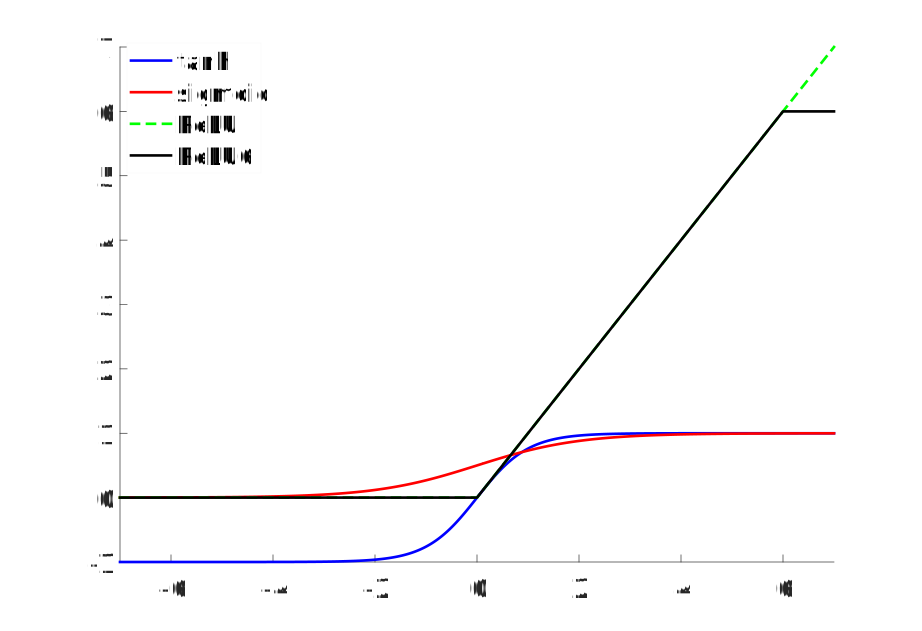
\includegraphics[width=0.9\textwidth]{actifun.pdf}
    \caption{Activation functions}
    \label{fig:acti}
\end{figure}
%
\subsubsection{Sigmoid and Hyperbolic Tangent (Tanh)}
$Sigmoid$ and $Tanh$ are smooth activation functions that limit the $\mathbb{R}$ domain into a narrower domain: $[0, 1]$ for $Sigmoid$, and $[-1, 1]$ for the $Tanh$, as shown in Figure \ref{fig:acti} \cite{matteucci_artificial_2019}. They can be described using Equations \eqref{eq:sigmoid} and \eqref{eq:tanh} \cite{krizhevsky_imagenet_2012}.
%
\begin{equation}
    h(x) = \frac{1}{1 + e^{-x}}
    \label{eq:sigmoid}
\end{equation}
%
\begin{equation}
    h(x) = \frac{e^{x} - e^{-x}}{e^{x} + e^{-x}}
    \label{eq:tanh}
\end{equation}
%
However, they saturate at the asymptotes, which means that their gradient is close to 0 outside the input range $[-4, 4]$ \cite{glorot_understanding_2010}. As the back-propagation algorithm (see Section \ref{subsec:train}) requires gradient multiplication, gradient far away from the output vanishes (close to 0) and deep models do not learn. It is the \textbf{vanishing gradient problem} \cite{khan_survey_2020, matteucci_artificial_2019, goodfellow_deep_2016, maas_rectier_2013}.
%
\subsubsection{ReLU and ReLU6}
In order to overcome this vanishing gradient problem, the Rectified Linear Unit (ReLU) which is defined by Equation \eqref{eq:relu} was developed by \textcite{krizhevsky_imagenet_2012}.
%
\begin{equation}
    h(x) = max(0, x)
    \label{eq:relu}
\end{equation}
%
This function increases the learning and computational speed compared to the $Tanh$ and $Sigmoid$ functions. It also improves the efficiency of the propagation gradient (avoiding vanishing or exploding gradient) \cite{abdelouahab_accelerating_2018, maas_rectier_2013}. However, some perceptrons can become inactive after learning. It means that their output is zero for all input. It is called the \textbf{dying neuron problem} which decreases the model capacity \cite{matteucci_artificial_2019}. A solution would be to use a derivative of the ReLU activation function designed to solve this problem such as leaky ReLU for example \cite{matteucci_artificial_2019, maas_rectier_2013}.

We can also use the dying neuron property to learn sparse features. It was done by \textcite{krizhevsky_convolutional_2010} by setting an upper bound to the ReLU output. For example, they chose to limit the output of the perceptron to 6, as described in Equation \eqref{eq:relu6}. This activation function is called ReLU6 because its output range is limited to $[0, 6]$. 
%
\begin{equation}
    h(x) = max(0, x, 6)
    \label{eq:relu6}
\end{equation}
%
ReLU6 has the advantage to be designed for fixed-point operations and quantization approaches (which will be described in Section \ref{subsec:mdopti}), instead of floating-point operations. It means the number of bits for the integer part can be limited to 3 bits because the output $ \in [0, 6]$ (with 3 bit, we can represent numbers in the range $[0, 2^3-1]$ = $[0, 7]$). The accuracy of the model can thus be increased by assigning the other available bits to the decimal part. This property makes ReLU6 to be used in models that aim mobile and embedded platforms like MobileNet \cite{howard_mobilenets_2017}. Indeed, fixed-point operations, especially on \acrshort{fpga}, are more efficient in terms of hardware utilization and power consumption \cite{david_hardware_2007}. In the frame of this thesis, the ReLU6 activation function is used.

